\documentclass[numbers=noendperiod,bibliography=totoc,paper=a4,pagesize,DIV=calc,headings=small,10pt]{scrreprt}

\usepackage[ngerman]{babel} % Sprachanpassungen
\usepackage{fixltx2e} % Einige Problemfälle von LaTeX2e
\usepackage{soul} % Zusätzliche Möglichkeiten der Textauszeichnung
\usepackage{graphicx} % Einbindung von Graphiken
\usepackage{listings}
\usepackage{color}
\usepackage{float}
\usepackage{hyperref}
\usepackage{amsmath}
\usepackage{textcomp}
\usepackage[utf8]{inputenc}

\definecolor{listgray}{rgb}{0.88,0.88,0.88} 
\definecolor{green}{rgb}{0,0.88,0} 
\definecolor{blue}{rgb}{0,0,0.88} 



\lstdefinelanguage{hc11}{%
    sensitive=false,
    morecomment=[l]{;},
    commentstyle=\color{green},
    keywordstyle=\color{blue},
    % Misc
    morekeywords={Section, switch include, equ, ds.w, ds.b},
    % Load
    morekeywords={LDAA, LDAB, LDD, LDX, LDY, LDS},
    % Store
    morekeywords={STAA, STAB, STD, STX, STY, STS},
    % Transfer
    morekeywords={TAB, TBA, TAP, TPA, TSX, TXS, TSY, TYS},
    % Exchange
    morekeywords={XGDX, XGDY},
    % Clear
    morekeywords={CLR, CLRA, CLRB},
    % Add & Sub
    morekeywords={ABA, ADDA, ADDB, ADDD, ABX, ABY, SUBA, SUBB, SUBD, ADCA, ADCB, SBCA, SBCB},
    % Mul & Div
    morekeywords={MUL, FDIV, IDIV},
    % Logic
    morekeywords={ANDA, ANDB, ORAA, ORAB, EORA, EORB},
    % Compare
    morekeywords={CBA, CMPA, CMPB, CPD, CPX, CPY},
    % 0 Test
    morekeywords={TST, TSTA, TSTB},
    % Jumps
    morekeywords={BRA, JMP, BEQ, BNE, BCC, BCS, BMI, BPL,BVS, BVC, BGT, BGE, BEQ, BLE, BLT, BHI, BHS, BEQ, BLS, BLO, BRCLR, BRSET},
    % Subroutines
    morekeywords={BSR, JSR, RTS},
    % Stack
    morekeywords={PSHA, PSHB, PSHX, PSHY, PULA, PULB, PULX, PULY}
}

\lstset{
    literate=%
        {Ö}{{\"O}}1
        {Ä}{{\"A}}1
        {Ü}{{\"U}}1
        {ß}{{\ss}}1
        {ü}{{\"u}}1
        {ä}{{\"a}}1
        {ö}{{\"o}}1,
    backgroundcolor=\color{listgray},
    breaklines=false,
    %columns=felxibile,
    breakatwhitespace=true, 
    keepspaces=true,
    numbers=left,
    tabsize=4,
    linewidth=1.2\textwidth,
    language=hc11,
    %xleftmargin=.2\textwidth,
    %xrightmargin=.2\textwidth,
    frame=tb,
    basicstyle=\ttfamily\footnotesize\bfseries
}




\pagenumbering{roman}
%
% Title Page
\subject{Mikroprozessor Workshop \\ Wintersemester 2019/2020}
\title{Vier Gewinnt auf dem \\ Motorola 68HC11 Prozessor}
\subtitle{Benutzer- und Programmierhandbuch}
\author{\textbf{Michael Persiehl (tinf102296)} \and \textbf{Guillaume Fournier-Mayer (tinf101922)} }

\date{\today{}, Hamburg\\[3cm]
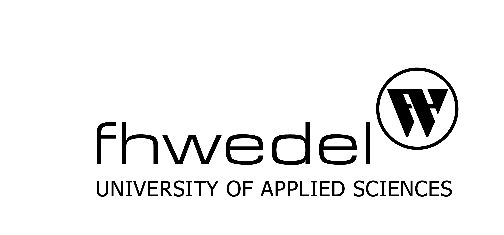
\includegraphics[scale=0.9]{img/fh_sw_RGB600dpi.eps}}


\pagestyle{headings}

\begin{document}
    \maketitle
    \tableofcontents
    \pagenumbering{arabic}

    \chapter{Benutzerhandbuch}
    \setcounter{page}{1}
    \section{Aufgabenstellung}
    Für den Mikroprozessor-Workshop im Wintersemester 2020 wurde das Spiel \textit{4 Gewinnt} auf dem Motorola 68HC11 Prozessor umgesetzt.
    Als Software wurde \textit{Geany} und als Compiler wurde \textit{miniIDE} unter Windows verwendet.
    \\
    Unser Ziel ist es \textit{4 Gewinnt} für zwei Spieler auf dem 68HC11 Board in Assembler zu programmieren.
    Für die Steuerung werden dabei die Tasten-, zur Anzeige der Spieldaten der LCD des Boards genutzt.
    \section{Spielregeln}
    Das Spiel wird auf einem 7 Felder breiten und 6 Felder hohen Spielbrett gespielt (Abbildung \ref{fig:spielfeld}),
    in das die Spieler abwechselnd ihre Spielsteine fallen lassen. Jeder Spieler besitzt 21 gleichfarbige Spielsteine (Spieler 1 komplett gefüllt, Spieler 2 innen leer. (Abbildung \ref{fig:spieler}))
    \begin{figure}[H]
        \centering
        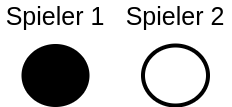
\includegraphics[scale=0.5]{img/spieler.png}    
        \caption{Spielsteine}
        \label{fig:spieler}
    \end{figure}
    Wenn ein Spieler einen Spielstein in eine Spalte fallen lässt, besetzt dieser den untersten freien Platz der Spalte.
    Gewinner ist der Spieler, der es als erster schafft, vier oder mehr seiner Spielsteine waagerecht, senkrecht oder diagonal in eine Linie zu bringen.
    Das Spiel endet unentschieden, wenn das Spielbrett komplett gefüllt ist, ohne dass ein Spieler eine Viererlinie gebildet hat.
    \begin{figure}[H]
        \centering
        \includegraphics[scale=0.5]{img/spielfeld.png}    
        \caption{Spielfeld}
        \label{fig:spielfeld}
    \end{figure}
    \section{Bedienung}
    Das Spiel wird mit vier Tasten gesteuert.
    Dabei wird der Cursor mit der linken und der rechten Taste, jeweils um eine eine Spalte in die gewünschte Richtung bewegt.
    Mit der unteren Taste wird ein Stein, an der aktuellen Cursorposition, in die Spalte geworfen.
    Über die Resettaste kann das komplette Spiel zurückgesetzt werden. Spieler 1 wäre nun wieder am Zug.
    \begin{figure}[H]
        \centering
        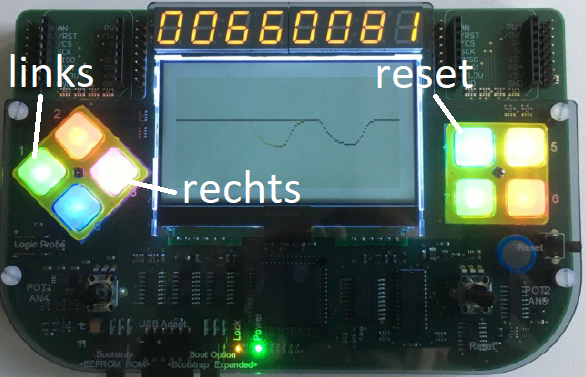
\includegraphics[scale=0.5]{img/board.png}    
        \caption{Board}
        \label{fig:board}
    \end{figure}

\section{Ausgabe}
    \subsection{Spielstart}
        Nach erfolgreichem Programmstart wird das leere Spielfeld in der Mitte des LCD's angezeigt.
        Links davon befindet sich ein Textfeld \textit{turn}, welches den Namen des Spielers anzeigt, der zurzeit dran ist.
        Beim Programmstart sowie beim Zurücksetzen des Spieles startet immer \textit{Spieler 1}.
        Unter dem Spielfeld ist der Cursor zu sehen, der zum Start des Spieles auf die mittlere Spalte zeigt.
    \subsection{Spielende}
        Falls ein Spieler gewonnen hat, wird unter dem Spielfeld der gewinnende Spieler angezeigt.
        Zusätzlich ist die Eingabe blockiert und das Spiel lässt sich nur mit den Resetbutton zurücksetzen.





    \section{Inbetriebnahme}
    Zum Ausführen des Spiels muss zuerst die Assemblerdatei in einer IDE wie z.B. Geany (Freeware: \url{https://www.geany.org/}) geöffnet werden (rote Markierung, Abbildung \ref{fig:geany}).
    \begin{figure}[H]
        \centering
        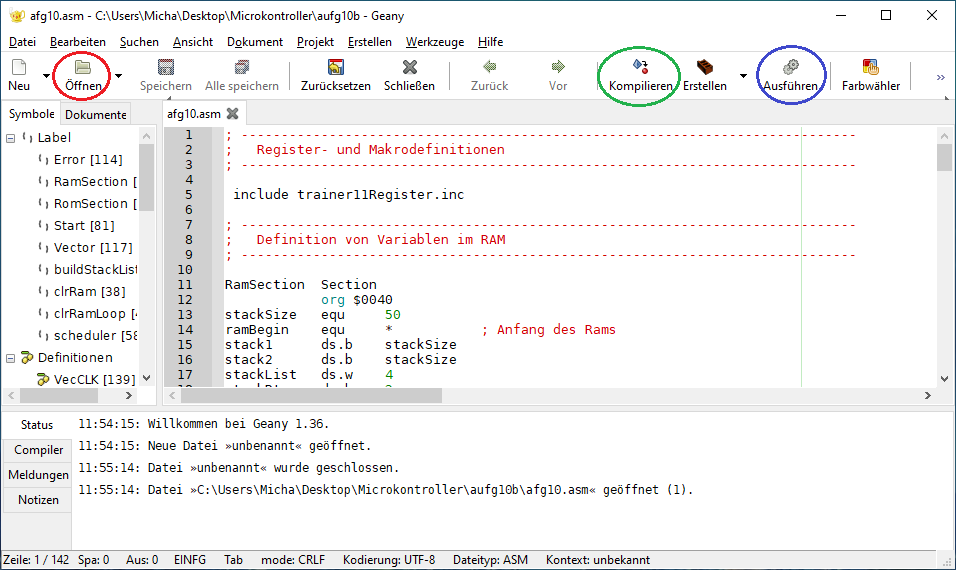
\includegraphics[scale=0.5]{img/geany.png}    
        \caption{Geany IDE}
        \label{fig:geany}
    \end{figure}
    Als nächstes müssen die Einstellungen in Geany geändert werden: 
    Zunächst der verwendete Kompiler, welchen wir von miniIDE nutzen, welche vorher im Verzeichnis \texttt{C:\textbackslash{}miniide} installiert sein muss (ansonsten muss der Pfad zum Kompiler später entsprechend angepasst werden).
    Ebenfalls wird die Software \textit{Realterm} in dem Verzeichnis \texttt{C:\textbackslash{}realterm} benötigt.
    \\
    Unter dem Stichwort \textit{Dokument} \textrightarrow{} \textit{Dateityp festlegen} \textrightarrow{} \textit{Kompilersprachen} muss \textit{Assembler} ausgewählt werden,
    danach im Menü-band unter \textit{Erstellen} erreicht man den Punkt \textit{Kommandos zum Erstellen konfigurieren} (Abbildung \ref{fig:geany-menu}).
    \begin{figure}[H]
        \centering
        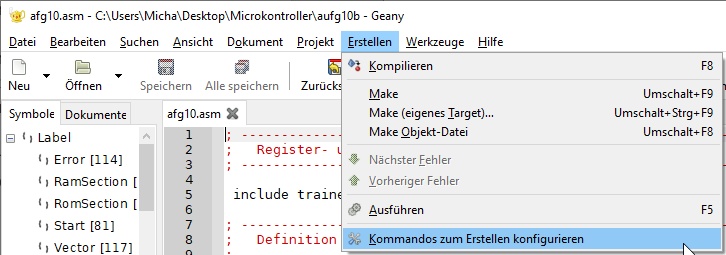
\includegraphics[scale=0.5]{img/geany-menu.png}    
        \caption{Geany IDE Menü}
        \label{fig:geany-menu}
    \end{figure}
    Hier muss nun unter \textit{Kommandos für ASM} folgendes eingetragen werden:
    \begin{center}
        \texttt{C:\textbackslash{}miniIDE\textbackslash{}ASM11 \%f -l}
    \end{center}
    und unter \textit{Befehle zum Ausführen}:
    \begin{center}
        \texttt{C:\textbackslash{}Realterm\textbackslash{}realterm "{}first"{} "{}display=1"{} "{}rows=40"{} "{}baud=9600"{} "{}sendfile=\%d\textbackslash{}\%e.s19"{}}
    \end{center}
    \begin{figure}[H]
        \centering
        \label{geany-config}
        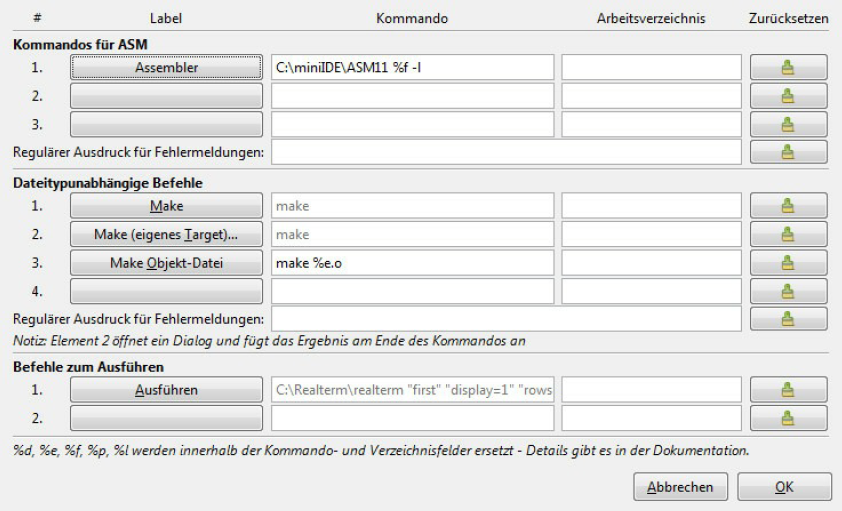
\includegraphics[scale=0.5]{img/geany-config.png}    
        \caption{Geany IDE Konfiguration}
    \end{figure}
    Gegebenenfalls muss hier noch \textit{Port=} mit der Nummer des entsprechenden COM-Ports ergänzt werden.
    \\
    Nach dem bestätigen per \textit{OK} müssen die Daten kompiliert und auf das Board überspielt werden (grüne und blaue Markierungen, Abbildung \ref{fig:geany}).
    Nach dem Klick auf \textit{Ausführen} öffnet sich jetzt \textit{Realterm} (Abbildung \ref{fig:realterm}). Nach Betätigung des Resetschalters können die Daten mit 
    \textit{Send File}, im Reiter \textit{Send}, ans Board übertragen werden. 
    \begin{figure}[H]
        \centering
        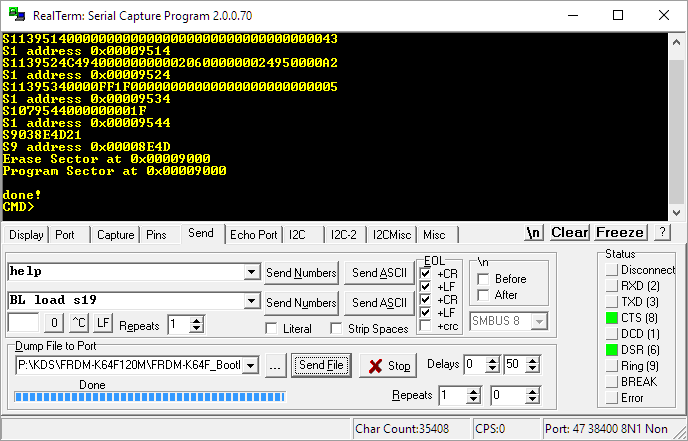
\includegraphics[scale=0.5]{img/realterm.png}    
        \caption{Realterm}
        \label{fig:realterm}
    \end{figure}


    \chapter{Programmiererhandbuch}
    \section{Spielfeld}
    In dem folgenden Kapitel wird das Spielfeld, dessen Aufbau in Zellen und die interne Repräsentation, 
    als Buffer, im Speicher erläutert.


    \subsection{Zelle}
        Eine Zelle wird auf dem LCD als Block von Pixeln betrachtet.
        Dabei besteht die Zelle aus folgender Formel:
        \begin{align}
        64 Pixel = 8 Pixel \cdot 8 Pixel
        \end{align}
        Diese 64 Pixel werden intern als acht hintereinander liegende Bytes repräsentiert.
        Dabei steht das erste Bit des ersten Bytes für den Pixel in der oberen linke Ecke.
        Um ein Pixel anzusteuern, wird das jeweilige Bit auf \textit{1} bzw. auf \textit{0} gesetzt.
        \begin{figure}[H]
            \centering
            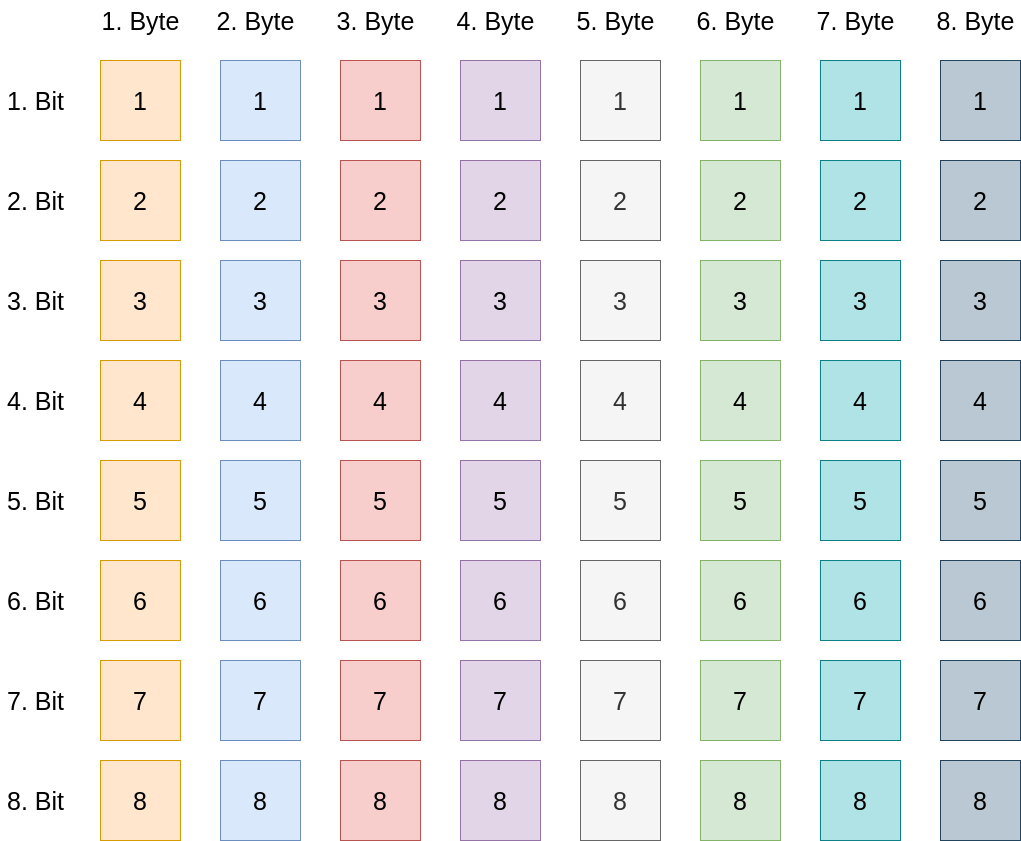
\includegraphics[scale=0.25]{img/zelle.png}    
            \caption{Darstellung einer Zelle im RAM}
        \end{figure}
    
    \subsubsection{Leere Zelle}
        Eine Leere Zelle ist jene, die kein Spielstein beinhaltet und somit nur aus Rand besteht.
        Um den vertikalen Rand darzustellen, müssen alle Bits des ersten und achten Bytes auf \textit{1} gesetzt werden.
        Für den horizontalen Rand müssen alle ersten und achten Bits des 2,3,4,5,6 und 7 Bytes auf \textit{1} gesetzt werden.
        \begin{figure}[H]
            \centering
            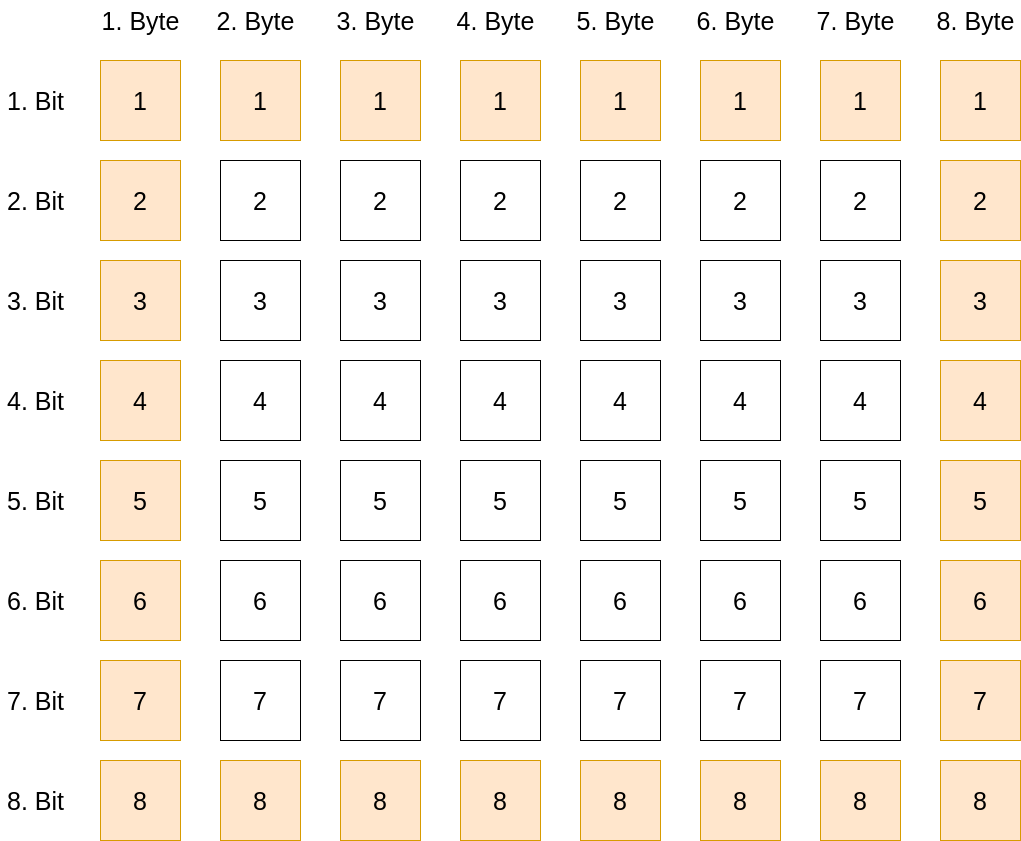
\includegraphics[scale=0.25]{img/leere-zelle.png}    
            \caption{Darstellung einer leeren Zelle im RAM}
        \end{figure}

    \subsubsection{Spieler 1 Zelle}
        Eine Zelle mit einem Spielstein von Spieler 1 ist jene, die aus Rand und aus einem gefüllten Spielstein besteht.
        \begin{figure}[H]
            \centering
            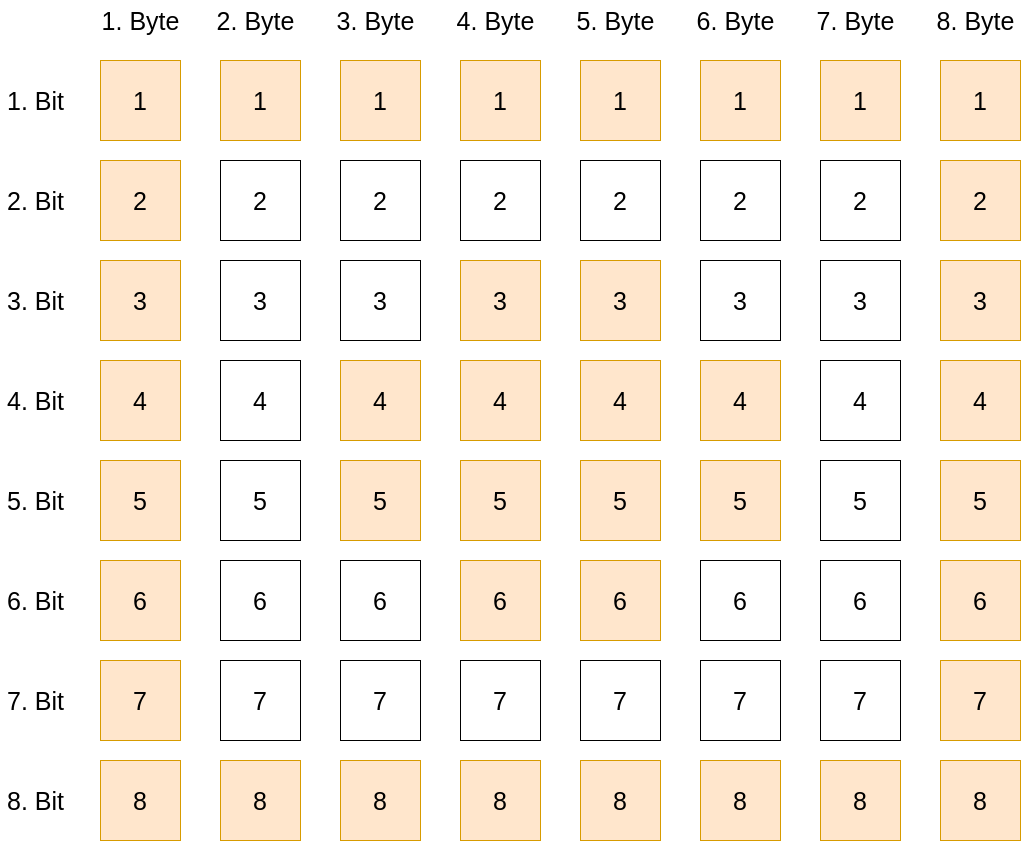
\includegraphics[scale=0.25]{img/spieler1-zelle.png}    
            \caption{Darstellung einer Zelle mit einem Spielstein von Spieler 1 im RAM}
        \end{figure}
    
    \subsubsection{Spieler 2 Zelle}
        Eine Zelle mit einem Spielstein von Spieler 1 ist jene, die aus Rand und aus einem leeren Spielstein besteht.
        \begin{figure}[H]
            \centering
            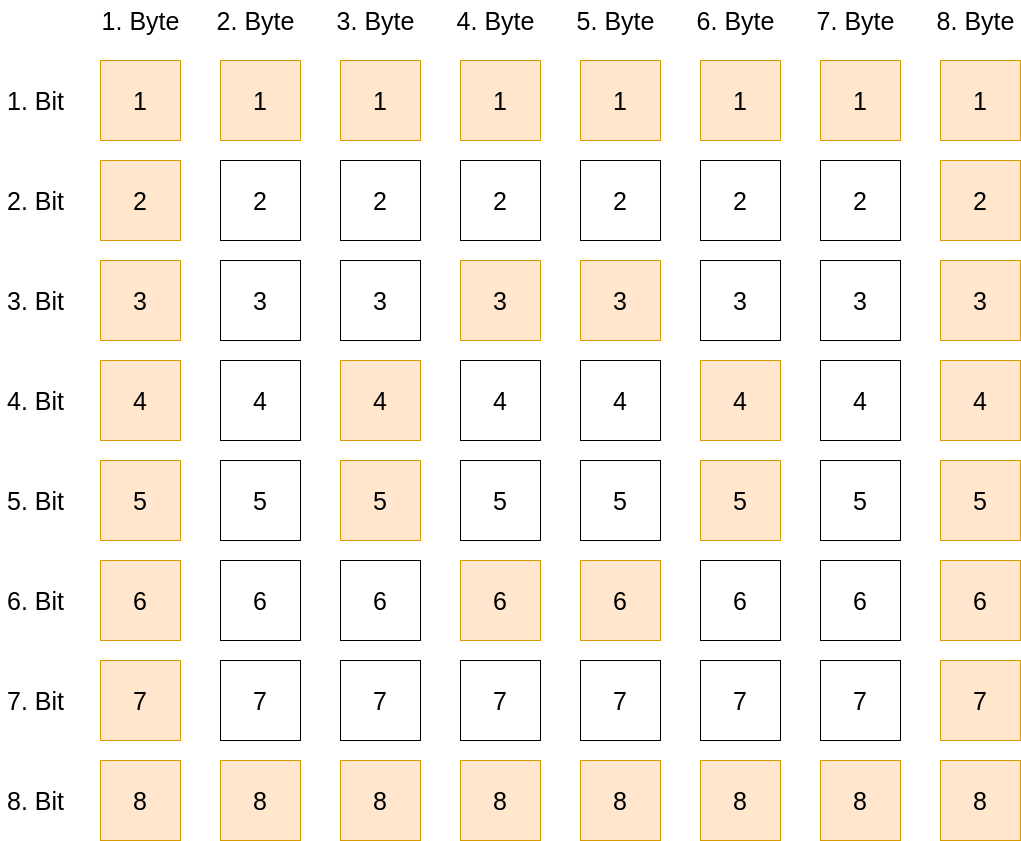
\includegraphics[scale=0.25]{img/spieler2-zelle.png}    
            \caption{Darstellung einer Zelle mit einem Spielstein von Spieler 2 im RAM}
        \end{figure}

    \subsection{Buffer}
        Das gesamte Spielfeld wird intern als Buffer repräsentiert.
        Änderungen am Spielfeld werden zunächst im Buffer getätigt, bevor der gesamte Inhalt an den LCD geschickt wird.
        \\
        Die Größe des Buffers berechnet sich dabei aus folgender Formel:
        \begin{align}
        Buffergr\ddot{o}sse = Zeilen \cdot Spalten \cdot Zellengr\ddot{o}sse
        \end{align}
        Da das Spielfeld aus sechs vertikalen Zellen und sieben horizontalen Zellen besteht und diese wiederrum aus acht Bytes bestehen,
        ergibt sich folgende Buffergröße:
        \begin{align}
        336 Byte = 6  \cdot 7  \cdot 8 Byte
        \end{align}

  





        

    \newpage
\section{Eingabe}\label{cha:input}
    In dem folgenden Kapitel wird die Eingabe durch Tastendruck, deren Entprellung und Flankenerkennung erläutert.
    
    \subsection{Tastenbyte auslesen}
        Um auf einen Tastendruck zu reagieren wird in regelmäßigen Abstand das \textit{PIO\_B}-Byte ausgelesen.
        Dabei ist dieses \textit{n-aus-8-Kodiert}. Jedes Bit repräsentiert dabei den Zustand einer Taste.
        Ist ein Bit auf 0 gesetzt, ist die Taste zurzeit gedrückt und umgekehrt.

        \begin{description}
            \item [Taste 0 (11111110)]
            Setzt abhängig davon wer zurzeit am Zug ist, einen entsprechenden Stein an der Cursorposition.
            Sobald der Stein gesetzt worden ist, wird die Logik angesteuert um einen möglichen Sieg zu ermitteln.
            \item [Taste 1 (11111101)] Bewegt den Cursor nach Links.
            \item [Taste 3 (11110111)] Bewegt den Cursor nach Rechts.
            \item [Taste 4 (11101111)] Setzt das Spiel zurück.
        \end{description}


    \subsection{Flankenerkennung und Entprellung}
        Da das Einlesen des \textit{PIO\_B}-Bytes in einer Schleife ausgeführt wird,
        muss sichergestellt werden, dass nur eine Flanke pro Tastendruck ausgewertet wird.
        Zusätzlich muss, durch die fehlende Hardwareentprellung der Tasten, die Entprellung in Software realisiert werden.
        \\
        \\
        Dazu wird zunächst das \textit{buttonFlag} getestet. Ist es nicht gesetzt, kann auf eine Taste reagiert und
        das Flag gesetzt werden. Ist es jedoch gesetzt, wird ein Timer inkrementiert.
        Ist dieser größer als 250, wird das \textit{buttonFlag} zurück gesetzt,
        welches es wieder ermöglicht auf einen Tastendruck zu reagieren.
        Falls der Timer jedoch kleiner als 250 ist, muss weiterhin gewartet werden und ein Entprellen der Tasten
        zu gewährleisten.

        \begin{figure}[H]
            \centering
            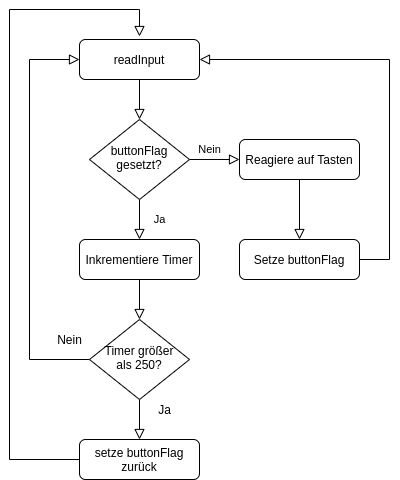
\includegraphics[scale=0.5]{img/entprellung.png}    
            \caption{Programmablaufplan: \textit{readInput}}
        \end{figure}

    \newpage
\section{Ausgabe}
    In diesem Kapitel wird erläutert wie die Ausgabe auf dem LCD realisiert wurde.
    Dabei werden die eigenheiten des Displays und die representation von Text innerhalb des Speichers erklärt.

    \subsection{LCD}
        Als Display steht dem Board ein \textit{NHD-C12864A1Z-FSW-FBW-HTT} zur Verfügung.
        Dieses besitzt 128 x 64 Pixel. Da der Cursor jedoch 8 Pixel hoch ist,
        bildet das LCD 128 Spalten und acht Zeilen ab.

    \subsection{Spielfeld}
        Um das Spielfeld zu zentrieren wird auf jede horizontale Berechnung die Konstante 
        \textit{boardOffset} addiert.\\
        Diese berechnet sich aus folgender Formel:
        \begin{equation}
            boardOffset = \dfrac{Displaybreite}{2} - \dfrac{Spielfeldbreite}{2}
        \end{equation}
        Konkret bedeutet das:
        \begin{equation}
            36 = \dfrac{128 Pixel}{2} - \dfrac{7 Zeilen \cdot 8 Pixel}{2}
        \end{equation}
        

    \subsection{Text}
        Da kein dynamischer Text für die Ausgabe benötigt wird, wird jeglicher Text aus dem Speicher 
        ausgelesen.
        \\
        Dabei besteht ein Buchstabe aus zwei bis vier Bytes. Zusätzlich wird ein Leerzeichen,
        in Form eines leeren Bytes, an das Ende des Buchstaben angefügt.
        \\\\
        Somit ergibt sich Beispielsweise folgende Bytefolge für den Buchstaben \textit{T}:
        \begin{center}
            \texttt{\$02,\$7E,\$02,\$00}    
        \end{center}
        Um nun eine Buchstabenfolge als Text auszugeben, wird die Länge dieser im ersten Byte gespeichert.
        Somit ist es möglich, in einer Schleife eine Buchstabenfolge auszugeben, ohne den dahinter liegenden
        Speicher mit auszulesen. Alternativ könnte hier auch ein Stopbyte verwendet werden.
        Dies hätte den Vorteil, dass auch Texte, die länger als 254 Zeichen lang sind, Ausgegeben werden können.
        \\
        Die folgende Tabelle zeigt die Kodierung mit dem Beispieltext \textit{Player}:
        \begin{center}
            \begin{tabular}{c | l}
                P: & \texttt{30,\$7E,\$12,\$12,\$0C,\$00}\\
                l: & \texttt{\$02,\$7E,\$00} \\
                a: & \texttt{\$20,\$54,\$54,\$78,\$00}\\ 
                y: & \texttt{\$1C,\$A0,\$A0,\$7C,\$00}\\ 
                e: & \texttt{\$38,\$54,\$54,\$48,\$00}\\ 
                r: & \texttt{\$7C,\$08,\$04,\$08,\$00}\\
                 : & \texttt{\$00,\$00}
            \end{tabular}
        \end{center}
      

    \newpage
\section{Cursor}
    In diesem Kapitel wird der Cursor mit allen Funktionen und Bestandteilen erläutert.
    Darunter fallen unter anderem eine Variable (cursorColumn, deklariert in Viergewinnt.asm, Größe 1 Byte)
    zur Beschreibung der horizontalen-Position auf dem Board, welche die Spalte, die durch den Cursor ausgewählt wird repräsentiert und eine Konstante
    (cursorRow, in Viergewinnt.asm deklariert, hat den Wert 6) für die vertikale-Position des Cursors direkt unterhalb des Spielfelds.

    \subsection{Aufbau}
        Der Cursor wird auf dem LCD durch einen 6 Byte Breiten, ausgefüllten Pfeil unter dem Spielfeld (Zeile 6) dargestellt (Abbildung 7).

        \begin{figure}[H]
            \centering
            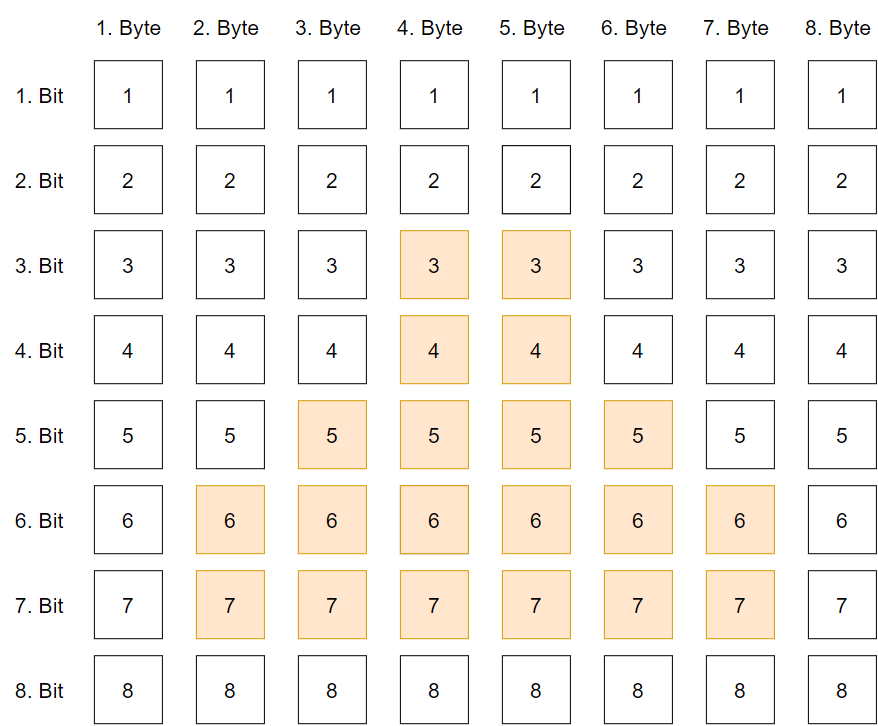
\includegraphics[scale=0.35]{img/cursor.png}    
            \caption{CAPTION}
        \end{figure}
    
    \subsection{Steuerung}
        Der Cursor startet nach betätigen des Resets (Taste 4 des Boards) oder bei Programmstart in der Mitte des Spielfeldes (Spalte 4).
        Er kann durch die Tasten 1 (nach links) und 3 (nach rechts) horizontal unter dem Spielfeld bewegt werden.
        Bei weiterer Bewegung und einer Cursorposition am Spielfeldrand erscheint der Cursor am gegenüberliegenden Spielfeldrand um schnelleres manövrieren zu ermöglichen (Abbildung 8).
        Bei Versersetzen des Cursors wird zuerst auf dem LCD der alte Cursor gelöscht,
        dann die Variable cursorColumn für links um 1 reduziert oder für rechts um 1 erhöht.
        Danach wird der Cursor erneut auf dem LCD an der geänderten cursorColumn angezeigt.

        \begin{figure}[H]
            \centering
            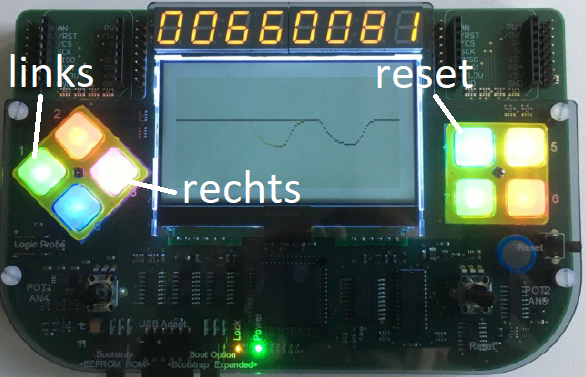
\includegraphics[scale=0.5]{img/board.png}    
            \caption{CAPTION}
        \end{figure}
    \newpage
\section{Logik}
    In dem folgenden Abschnitt wird die Spiellogik bzw. die genutzten Algorithmen im Detail erläutert.
    Darunter fallen Unterprogramme zur Adressberechnung, zum Prüfen, ob eine Zelle leer ist, zum Spielerwechsel,
    zum Feststellen der Länge einer Steinfolge sowie zum Feststellen des Spielendes.

    \subsection{Umrechnung der Boardadresse in eine Bufferadresse}
        Da das Spielfeld im Buffer Zeilenweise hintereinander weg verläuft, also alle 42 Zellen hintereinander liegen,
        aber auf dem Display die Zeilen untereinander angeordnet sind, müssen die Koordinaten umgerechnet werden können.
        \\
        Zum umrechnen einer Spielfeldkoordinate wird folgende Formel verwendet:
        \begin{align}
            Addresse = (Spalte \cdot 8) + (Zeile \cdot 56)
        \end{align}
        Die Multiplikatoren ergeben sich aus einer Zellenhöhe von 8 für die Zeilenzahl und aus einer Zellenbreite von 8 bei 7 Zellen pro Zeile = 56.
        Also bei einer Spielfeldkoordinate bei Spalte 3 und Zeile 2 währe die Berechnung folgende:
        \begin{align}
            136 = (3 \cdot 8) + (2 \cdot 56) 
        \end{align}
        

    \subsection{Prüfen des Zelleninhalts}
        Um feststellen zu können, ob ein Spieler eine zusammenhängende Steinfolge besitzt,
        muss es nicht nur möglich sein zu erkennen, ob eine Zelle leer oder belegt ist,
        sondern ebenfalls von welchem Spieler ein Stein ist.
        \\
        Dazu wird erst im 3. Byte der Zelle (der Rand eines eventuellen Spielsteins für beide Varianten)
        geprüft, ob nur Nullen (leere Zelle) oder auch Einsen (ein Spielstein von Spieler 1 oder Spieler 2) vorhanden sind.
        \\
        Wenn ein Spielstein gefunden wurde,
        wird danach geprüft, ob in der Mitte des Steins Einsen vorhanden sind (ausgefüllter Spielstein) oder nicht (innen leer)
        um ihn einem Spieler zuzuordnen.

        \begin{figure}[H]
            \centering
            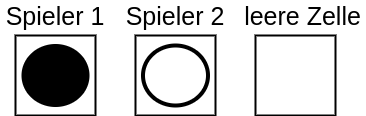
\includegraphics[scale=0.5]{img/steine.png}    
            \caption{Zellenbelegung}
        \end{figure}

    \subsection{Spielerwechsel}
        Zum Wechsel des Spielers wird der aktuelle Spieler aus der Variable „player“ ausgelesen (Spieler 1 oder Spieler 2).
        Danach wird dann auf den jeweils anderen Spieler gewechselt.

        \begin{figure}[H]
            \centering
            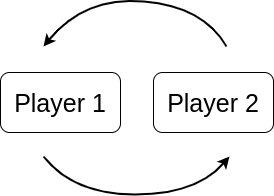
\includegraphics[scale=0.5]{img/spielerwechsel.png}    
            \caption{Spielerwechsel}
        \end{figure}


    \subsection{Feststellen der Anzahl an zusammenhängenden Steinen}
        Da der Zustand eines gewonnenen Spiels nur direkt nach dem setzen eines Steins vorkommen kann,
        wird direkt nach jedem Zug darauf geprüft.
        \\
        Um festzustellen wie viele Steine zusammenhängend vom gleichen Spieler sind,
        werden immer von dem neu gelegten Stein zwei gegenüberliegende Seiten geprüft.
        Um die Gesamtzahl zu bestimmen muss am Ende noch eins abgezogen werden,
        damit der neu gelegte Stein nicht doppelt gezählt wird.

        \begin{figure}[H]
            \centering
            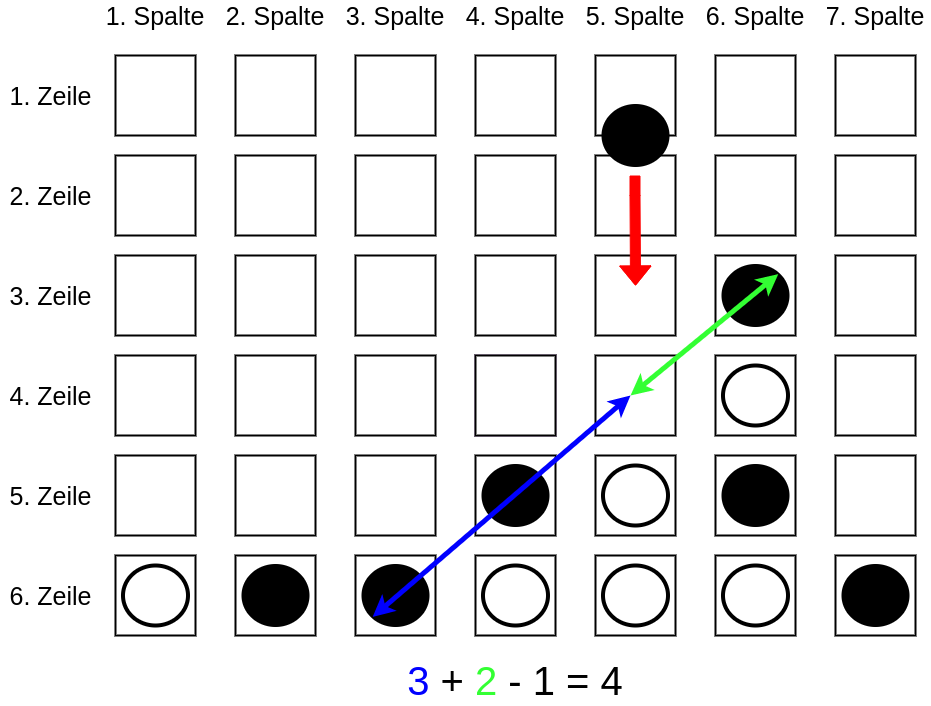
\includegraphics[scale=0.3]{img/gewinnbedingung.png}    
            \caption{Zusammenhängende Steine}
        \end{figure}

        Eine Ausnahme bilden die Richtungen oben und unten.
        Da über dem neugelegten Stein keine weiteren Steine sein können, wird nur nach unten geprüft.
        \\
        Wenn bei dem Zählen der zusammenhängenden Steine mehr als vier erkannt werden,
        bedeutet dies das Spielende und es wird die Variable \textit{playerWonFlag} auf 1 gesetzt um anschließend weitere Spielzüge zu sperren.

    \subsection{Main Loop}
        In dem \textit{MainLoop} wird per Schleife ständig das Datenbyte der Tasten ausgelesen.
        Dieses polling wird durch den konstanten Aufruf des Unterprogramms \textit{readInput} realisiert (siehe Kapitel \ref{cha:input}).
        Solange keine Taste betätigt ist, wird der Rest des Unterprogramms übersprungen und nur das Auslesen des Datenbytes durchgeführt.
      
    \newpage
\chapter{Listening}


\begin{center}
    \lstinputlisting{../src/Viergewinnt.asm}    
\end{center}


    \listoffigures
    \listoftables
    
\end{document}
